% -*- coding: UTF-8; -*-
\documentclass[11pt]{article}

\usepackage[utf8]{inputenc}
\usepackage[english]{babel}

\usepackage[top=2cm, bottom=2cm, left=2cm, right=2cm, columnsep=20pt]{geometry}  
\usepackage{graphicx}      
\usepackage{url}           
\usepackage{fancyvrb}      
\usepackage{amsmath}
\usepackage{cancel}
\usepackage[usenames]{color}
\usepackage{mathrsfs}
\usepackage{amssymb}
\usepackage{mathtools}
\usepackage{xfrac}
\usepackage{float}
\usepackage{wrapfig}
\usepackage{framed}
\usepackage{subcaption}
\usepackage{listings}
\allowdisplaybreaks

\newcommand{\Var}[1]{\mathrm{Var}\!\left[#1 \right]}
\newcommand{\Bias}[1]{\mathrm{Bias}\!\left[#1 \right]}
\newcommand{\Expect}[2][]{\mathbb{E}_{#1}\!\left[#2 \right]}
\newcommand{\sigmoid}[1]{\mathrm{sigmoid}\left(#1 \right)}
\newcommand{\KL}[1]{\mathrm{KL}\left( #1 \right)}

\newcommand{\diff}{\mathrm{d}}

\begin{document}

\begin{titlepage} % Suppresses displaying the page number on the title page and the subsequent page counts as page 1
	\newcommand{\HRule}{\rule{\linewidth}{0.5mm}} % Defines a new command for horizontal lines, change thickness here
	
	\center % Centre everything on the page
	\vspace*{2cm}
	
	%------------------------------------------------
	%	Headings
	%------------------------------------------------
	
	\textsc{\LARGE Universit\'e de Montr\'eal}\\[1cm] % Main heading such as the name of your university/college
	\textsc{\Large IFT6269 - Probabilistic Graphical Models}\\[2cm] % Major heading such as course name
		
	%------------------------------------------------
	%	Title
	%------------------------------------------------
	
	\HRule\\[0.5cm]
	{\huge\bfseries Homework 5}\\[0.2cm] % Title of your document
	\HRule\\[3cm]
	
	%------------------------------------------------
	%	Author(s)
	%------------------------------------------------
	
	{\large\textit{Author}}\\
	 Patrice \textsc{B\'echard}\\ % Your name
	 20019173
	
	%------------------------------------------------
	%	Date
	%------------------------------------------------
	
	\vfill\vfill\vfill % Position the date 3/4 down the remaining page
	
	{\large\today} % Date, change the \today to a set date if you want to be precise
	
	%------------------------------------------------
	%	Logo
	%------------------------------------------------
	
	%\vfill\vfill
	%
\includegraphics[width=0.2\textwidth]{~/placeholder.jpg}\\[1cm] % Include a department/university logo - this will require the graphicx package
	 
	%----------------------------------------------------------------------------------------
	
	\vfill % Push the date up 1/4 of the remaining page
	
\end{titlepage}

%------------------------------------------------------
%		Num 1
%------------------------------------------------------

\section{Cautionary tale about importance sampling}\label{sec:num1}

Suppose that we wish to estimate the normalizing constant $Z_p$ for an un-normalized Gaussian ${\tilde{p}(x) = \exp \left( - \frac{1}{2\sigma_p ^2} x^2 \right)}$; i.e. we have $p(\cdot) \sim \mathcal{N}(0, \sigma_p ^2)$ with $p(x) = \tilde{p}(x)/Z_p$. Given $N$ i.i.d samples $x^{(1)}, \dots , x^{(N)}$ from a standard normal $q(\cdot) \sim \mathcal{N}(0,1)$, consider the importance sampling estimate :

\begin{align*}
\hat{Z} = \frac{1}{N} \sum_{i=1} ^{N} \frac{\tilde{p}(x^{(i)})}{q(x^{(i)})}
\end{align*}


\begin{description}
%--------------------------- num 1, question a -------------
\item [(a)] We can show that $\hat{Z}$ is an unbiased estimator of $Z_p$. First let's develop the expression of the expectation value of $\hat{Z}$ :

\begin{align*}
\Expect[q]{\hat{Z}} & = \Expect[q]{ \frac{1}{N} \sum_{i=1} ^{N} \frac{\tilde{p}(x^{(i)})}{q(x^{(i)})}} \\
								 & = \frac{1}{N} \Expect[q]{\sum_{i=1} ^{N} \frac{\tilde{p}(x^{(i)})}{q(x^{(i)})}} \\
								 & = \frac{1}{N} \sum_{i=1} ^{N} \Expect[q]{ \frac{\tilde{p}(x^{(i)})}{q(x^{(i)})}} \\
								 & = \frac{1}{N} \sum_{i=1} ^{N} \left( \int_x \frac{\tilde{p}(x^{(i)})}{\cancel{q(x^{(i)})}} \cancel{q(x^{(i)})} \diff x \right) \\
								 & = \frac{1}{N} \sum_{i=1} ^{N} \left( \underbrace{\int_x \tilde{p}(x^{(i)})\diff x}_{Z_p} \right) && \text{ because } \int_x p(x)\diff x = \int_x \frac{\tilde{p}(x)}{Z_p} \diff x = 1 \\
								 & = \frac{1}{\cancel{N}} \left(\cancel{N} Z_p\right) \\
								 & = Z_p
\end{align*}

We know that the formula to compute the bias of an estimator is :

\begin{align*}
\Bias{\hat{\theta}} = \Expect{\hat{\theta}} - \theta
\end{align*}

For our case, we thus have :

\begin{align*}
\Bias{\hat{Z}} = \Expect{\hat{Z}} - Z_p = Z_p - Z_p = 0
\end{align*}

We thus have shown that $\hat{Z}$ is an unbiased estimator of $Z_p$. $\blacksquare$


%--------------------------- num 1, question b ------------- 
\item [(b)] Letting $f(x) := \tilde{p}(x)/q(x)$, we can show that $\Var{\hat{Z}} = \frac{1}{N} \Var{f(x)}$ whenever $\Var{f(x)}$ is finite. To do so, let's develop the expression for the variance of $\hat{Z}$ :

\begin{align*}
\Var{\hat{Z}} & = \Expect{\left( \hat{Z} - \Expect{\hat{Z}} \right)^2} \\
			  & = \Expect{\left( \frac{1}{N}\sum_{i=1}^{N} f \left(x^{(i)}\right) - \Expect{ \frac{1}{N}\sum_{i=1}^{N} f \left(x^{(i)} \right)} \right)^2} \\
			  & = \Expect{\left( \frac{1}{N}\sum_{i=1}^N f \left( x^{(i)} \right) - \frac{1}{N} \sum_{i=1}^N \Expect{f \left( x^{(i)} \right)} \right)^2} \\
			  & = \Expect{\left( \frac{1}{N} \sum_{i=1}^N \left( f\left( x^{(i)} \right) - \Expect{f\left( x^{(i)} \right)}  \right) \right)^2} \\ 
			  & = \frac{1}{N^2} \Expect{ \sum_{i,j = 1}^N \left\langle f\left( x^{(i)} \right) - \Expect{f\left( x^{(i)} \right)} , f\left( x^{(j)} \right) - \Expect{f\left( x^{(j)} \right)} \right\rangle} \\
			  & = \frac{1}{N^2} \sum_{i,j = 1}^N \Expect{\left\langle f\left( x^{(i)} \right) - \Expect{f\left( x^{(i)} \right)} , f\left( x^{(j)} \right) - \Expect{f\left( x^{(j)} \right)} \right\rangle} \\
			  & = \frac{1}{N^2}\sum_{i = 1}^N \underbrace{\Expect{\left( f\left( x^{(i)} \right) - \Expect{f\left( x^{(i)} \right)} \right)^2}}_{\Var{f\left( X \right)}} \\
			  & = \frac{1}{N^2} N \:\Var{f(X)} \\ 
			  & = \frac{1}{N} \Var{f(X)} \qquad\blacksquare
\end{align*}






%--------------------------- num 1, question c -------------
\item [(c)] To find for which values of $\sigma_p ^2$ is the variance $\Var{f(x)}$ finite, let's develop the expression for $f(x)$ :

\begin{align*}
f(x)  = \frac{\tilde{p}(x)}{q(x)} & = \frac{\exp \left( - \frac{1}{2\sigma_p ^2} x^2 \right)}{\frac{1}{\left( 2\pi \right)^{d/2}} \exp \left( -\frac{1}{2}x^2 \right)} \\
								  & = \left(2\pi \right)^{d/2} \exp \left( - \frac{1}{2\sigma_p ^2} x^2 + \frac{1}{2}x^2 \right) \\
								  & = \left(2\pi \right)^{d/2} \exp \left( - \frac{1}{2}x^2 \left( \frac{1}{\sigma_p ^2} - 1 \right) \right)
\end{align*}

We notice that $f(x)$ is in fact an un-normalized Gaussian itself with variance $\left( \frac{1}{\sigma_p ^2} - 1 \right)^{-2}$. The value of the variance diverges when $\sigma_p ^2 = 1$. The variance of $f(x)$ is thus finite for all values of $\sigma_p~^2~\in~\mathbb{R}^+~\backslash~\{1\}$.





\end{description}
\clearpage

%------------------------------------------------------
%		Num 2
%------------------------------------------------------

\section{Gibbs sampling and mean field variational inference}\label{sec:num2}

We consider the Ising model with binary variables $X_s \in \{0,1\}$ and a factorization of the form:

\begin{align}\label{eq:dist_p}
p(x;\eta) = \frac{1}{Z_p} \exp \left( \sum_{s \in V} \eta_s x_s + \sum_{\{s,t\} \in E} \eta_{st} x_s x_t \right)
\end{align}

We also consider the $7 \times 7$ 2D grid as shown here :

\begin{figure}[htbp]
\begin{center}
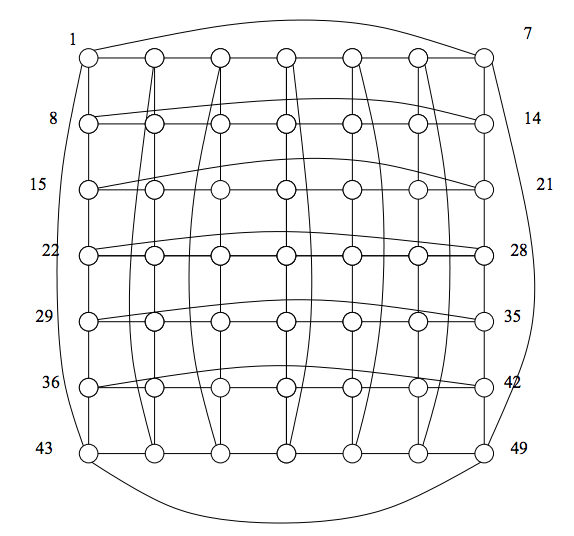
\includegraphics[scale=0.6]{figures/ising_grid.png}
\caption{The undirected graphical model considered.}
\label{fig:ising}
\end{center}
\end{figure}

We will consider approximate inference methods to approximate the node marginal moments $\mu_s := p(X_s = 1)$ in this model.


\begin{description}
%--------------------------- num 2, question a -------------
\item [(a)]

First, we will use Gibbs sampling to estimate the node marginal moments $\mu_s := p(X_s = 1)$. To do so, we have to derive the Gibbs sampling updates for this model. We know that the distribution from which we sample each $x_s$ is given by : 

\begin{align*}
p(x_i = 1 \mid x_{\neg i} ) & \propto p\left(x_i, x_{\neg i}\right) \\
							& = \exp \left( \eta_i \underbrace{x_i}_{=1} + \sum_{j \in N(i)} \eta_{ij} \underbrace{x_i}_{=1} x_j + \underbrace{\mathrm{rest}}_{=0} \right) && N(i) \text{ : neighbors of node i} \\
							& = \exp \left( \eta_i + \sum_{j \in N(i)} \eta_{ij} x_j\right)
\end{align*}

We re-normalize to get the conditional :

\begin{align*}
p(x_i=1\mid x_{\neg i}) & = \frac{\exp \left( \eta_i + \sum_{j \in N(i)} \eta_{ij} x_j\right)}{\underbrace{1}_{p(x_i=0\mid x_{\neg i})} + \exp \left( \eta_i + \sum_{j \in N(i)} \eta_{ij} x_j\right)}\\
						& = \frac{1}{1 + \exp \left(-( \eta_i + \sum_{j \in N(i)} \eta_{ij} x_j)\right)} \\
						& = \sigmoid{\eta_i + \sum_{j \in N(i)} \eta_{ij} x_j}
\end{align*}

This is our update for this model. We will only have to generate a random number from $\text{Unif}[0,1]$ and see if its value is smaller than $p(x_i=1\mid x_{\neg i})$. If so, the node takes the value of 1 for this iteration, else it takes the value of 0. The class \texttt{IsingGibbs} in the file \texttt{hwk5.ipynb} is the implementation of the algorithm with cyclic sequential traversal of the nodes with given parameters. The method \texttt{\_gibbs\_sampling\_epoch} does the update over each node of the model once. The method \texttt{gibbs\_sampling} calls the \texttt{\_gibbs\_sampling\_epoch} method 1000 times for a burn-in period, then calls it 5000 more times, collecting a sample vector of the state of the model each time. At the end of the iterations, it uses the 5000 samples to form Monte Carlo estimates $\hat{\mu}_s$ of the moments $\Expect{X_s}$ at each node. Figure \ref{fig:gibbs_mean} present the estimates obtained for each node using a colormap to present the data. We repeat this whole process 10 times and use the estimates $\hat{\mu}_s$ to estimate the empirical standard deviation at each node. Figure \ref{fig:gibbs_std} presents the estimates the same way we did for figure \ref{fig:gibbs_mean}. Numerical values of each figure are presented in the appendix.

\begin{figure}[htbp]
\begin{center}
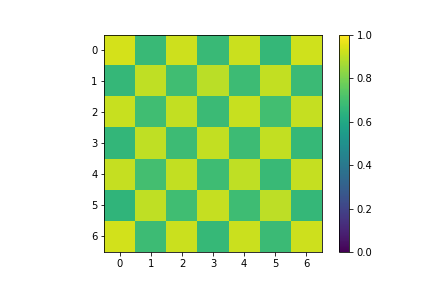
\includegraphics[scale=0.6]{figures/mean_gibbs.png}
\caption{Estimates $\hat{\mu}_s$ of the moments $\Expect{X_s}$ at each node of the Ising model using Gibbs sampling.}
\label{fig:gibbs_mean}
\end{center}
\end{figure}

\begin{figure}[htbp]
\begin{center}
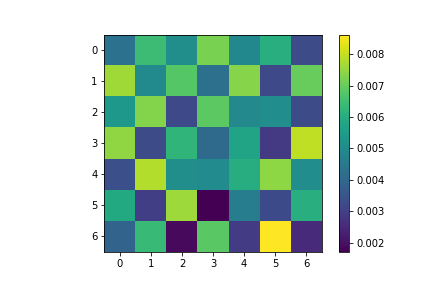
\includegraphics[scale=0.6]{figures/stddev_gibbs.png}
\caption{Empirical standard deviation of the estimates $\hat{\mu}_s$ of the moments $\Expect{X_s}$ at each node of the Ising model using Gibbs sampling.}
\label{fig:gibbs_std}
\end{center}
\end{figure}



%--------------------------- num 2, question b -------------
\item [(b)]

We will now use the naive mean field approximation to estimate the node marginal moments ${\mu_s := p(X_s = 1)}$.

First, let's derive the naive mean field updates, based on a fully factorized approximation, where we use the notation $q(X_s=1) = \tau_s$. We first develop the log-likelihood of $p(Z\mid \eta)$ :

\begin{align*}
\log p(z\mid \eta) & = \log \left[ \sum_x p(x,z \mid \eta) \right]\\
				   & = \log \left[\sum_x q(x) \frac{p(x,z \mid \eta)}{q(x)}\right] \\
				   & = \log \left[ \Expect[q]{\frac{p(x,z \mid \eta)}{q(x)}} \right] \\
				   & \geq \Expect[q]{\log \left[ \frac{p(x,z \mid \eta}{q(x)} \right]} && \text{by Jensen's inequality} \\
				   & = \mathcal{L}(q,\eta)
\end{align*}

We have now defined an evidence lower bound, which we now use to substract from the original log probability :

\begin{align*}
\log p(z \mid \eta) - \mathcal{L}(q,\eta) & = \log p(z \mid \eta) - \Expect[q]{\log \left[ \frac{p(x,z \mid \eta)}{q(x)} \right]} \\
										  & = \Expect[q]{\log p(z\mid \eta)} - \Expect[q]{\log \left[\frac{p(x,z \mid \eta)}{q(x)}\right]} \\
										  & = \Expect[q]{\log \frac{q(x)p(z\mid \eta)}{p(x,z\mid \eta)}} \\ 
										  & = \Expect[q]{\log \frac{q(x)}{p(x\mid z,\eta)}} \\
										  & = \KL{q(x) || p(x\mid z)}							  
\end{align*}

Our goal is to find $q$ such that the KL divergence is minimized. The mean field approximation is that we assume $q(x) = q(x_1,\dots,x_m)$ factorizes as $q(x) = \prod_{s \in V} q(x_s)$. We also know that the distribution of $p$ is given by equation \ref{eq:dist_p}. To update a certain $q_i$, we fix all other $q_j$ for $j \neq i$, and we optimize the KL divergence with respect to $q_i$.

\begin{align}\label{eq:partial_kl}
\KL{q||p} & = \Expect[q]{\log \frac{q(x)}{p(x|z)}} \nonumber\\
		  & = \Expect[q]{\log q(x) - \log p(x|z)} \nonumber\\
		  & = \sum_x q(x)\log q(x) - \Expect[q]{\log \left(\frac{1}{Z_p} \exp \left( \sum_{s \in V} \eta_s x_s + \sum_{\{s,t\} \in E} \eta_{st} x_s x_t \right) \right)} \nonumber\\
		  & = \sum_{s \in V} \left( \sum_{x} q(x_s)\log q(x_s) \right) - \underbrace{\Expect[q]{\sum_{s \in V} \eta_s x_s + \sum_{\{s,t\} \in E} \eta_{st} x_s x_t}}_{*} + \underbrace{\Expect[q]{\log Z_p}}_{\log Z_p}
\end{align}

Let's develop the (*) part independently :

\begin{align*}\label{eq:partial_edges}
\Expect[q]{\sum_{s \in V} \eta_s x_s + \sum_{\{s,t\} \in E} \eta_{st} x_s x_t} & = \Expect[q_i]{\sum_{s \in V} \eta_s \Expect[q_{\neg i}]{x_s} + \sum_{\{s,t\} \in E} \eta_{st} \Expect[q_{\neg i}]{x_s x_t}} \\
																			   & = \Expect[q_i]{\eta_i x_i + \sum_{j \neq i} \eta_j \Expect[q_{\neg i}]{x_j} + \sum_{j \in N(i)} \eta_{ij} \Expect[q_{\neg i}]{x_i x_j} + \underbrace{\text{rest}}_{\text{no } x_i}} \\
																			   & = \Expect[q_i]{\eta_i x_i + \sum_{j \neq i} \eta_j \tau_j + \sum_{j \in N(i)} \eta_{ij} x_i \tau_j + \underbrace{\text{rest}}_{\text{no } x_i}}
\end{align*}

We can now put back the (*) part in the KL calculation and derivate with respect to $q_i$ :

\begin{align*}
\frac{\partial}{\partial q_i} \KL{q||p} & = \frac{\partial}{\partial q_i} \left[ \sum_{s \in V} \left( \sum_{x} q(x_s)\log q(x_s) \right) - \Expect[q_i]{\eta_i x_i + \sum_{j \neq i} \eta_j \tau_j + \sum_{j \in N(i)} \eta_{ij} x_i \tau_j + \text{rest}} + \log Z_p \right] \\
										& = \log q(x_i) + 1 - \eta_i x_i - x_i \sum_{j \in N(i)} \eta_{ij} \tau_j \\
										& = 0
\end{align*}

We can now solve for $q(x_i)$ :

\begin{align*}
q^{(t+1)}(x_i) \propto \exp \left( \eta_i x_i + x_i \sum_{j \in N(i)} \eta_{ij} \tau_j ^{(t)} \right)
\end{align*}

And finally, since $x_i$ can take two values and that we only want the update for $q(x_i=1) = \tau_i$, we find the value we are looking for by normalizing :

\begin{align*}
\tau_i ^{(t+1)} & = \frac{\exp \left(  \eta_i (1) + (1) \sum_{j \in N(i)} \eta_{ij} \tau_j ^{(t)} \right)}{\exp \left(  \eta_i (0) + (0) \sum_{j \in N(i)} \eta_{ij} \tau_j ^{(t)} \right) + \exp \left(  \eta_i (1) + (1) \sum_{j \in N(i)} \eta_{ij} \tau_j ^{(t)} \right)} \\
				& = \frac{\exp \left(  \eta_i + \sum_{j \in N(i)} \eta_{ij} \tau_j ^{(t)} \right)}{1 + \exp \left(  \eta_i + \sum_{j \in N(i)} \eta_{ij} \tau_j ^{(t)} \right)} \\
				& = \sigmoid{ \eta_i + \sum_{j \in N(i)} \eta_{ij} \tau_j ^{(t)}}
\end{align*}

Let's now derive the expression of $\KL{q||p} - \log(Z_p)$, which we will use to monitor the progress of the model until convergence by plotting this value as a function of the number of epochs. We have already done the majority of the work previously, so let's start from \ref{eq:partial_kl}:

\clearpage

\begin{align*}
\KL{q||p} - \log Z_p & = \sum_{s \in V} \left( \sum_{x} q(x_s)\log q(x_s) \right) - \Expect[q]{\sum_{s \in V} \eta_s x_s + \sum_{\{s,t\} \in E} \eta_{st} x_s x_t} + \cancel{\log Z_p} - \cancel{\log Z_p} \\
					 & = \sum_{s \in V} \left(\tau_s \log \tau_s + (1-\tau_s)\log(1-\tau_s) \right) - \sum_{s \in V} \eta_s \tau_s - \sum_{\{s,t\} \in E} \eta_{st} \tau_s \tau_t
\end{align*}

Figure \ref{fig:kl_mean_field} presents the evolution for $\KL{q||p} - \log Z_p$ as a function of the number of epochs for 10 different random initializations of the grid.

\begin{figure}[htbp]
\begin{center}
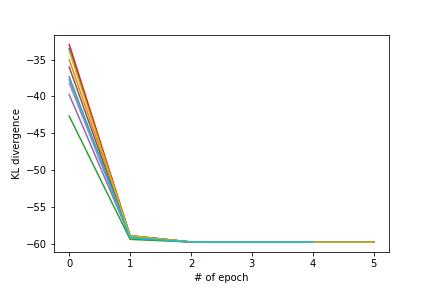
\includegraphics[scale=0.75]{figures/kl_div_mean_field.png}
\caption{Progress of expression $\KL{q||p} - \log Z_p$ as a function of the number of epochs for 10 different random initializations of the grid using the mean field approximation for variational inference of the node marginal moments in the model.}
\label{fig:kl_mean_field}
\end{center}
\end{figure}

We see that the KL divergence always converges to extremely similar values after between 2 and 5 iterations, which is much faster that the Gibbs sampling method. We can once again plot the estimates for each node using a colormap to present the data and repeat the process 10 times and use the estimates $\hat{\tau}$ to estimate the empirical standard deviation at each node. Figures \ref{fig:mean_field_mean} and \ref{fig:mean_field_std} presents both cases, respectively. Numerical values of each figure are presented in the appendix.

\begin{figure}[htbp]
\begin{center}
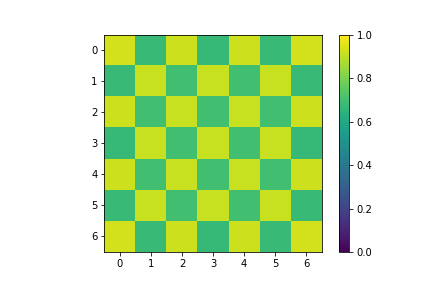
\includegraphics[scale=0.6]{figures/grid_mean_field.png}
\caption{Estimates $\hat{\mu}_s$ of the moments $\Expect{X_s}$ at each node of the Ising model using variational inference.}
\label{fig:mean_field_mean}
\end{center}
\end{figure}

\begin{figure}[htbp]
\begin{center}
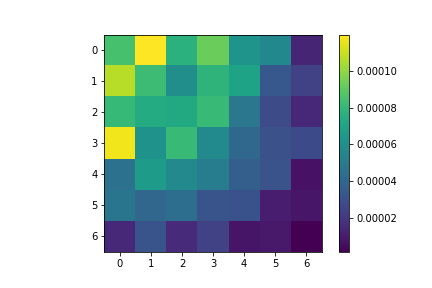
\includegraphics[scale=0.6]{figures/stddev_mean_field.png}
\caption{Empirical standard deviation of the estimates $\hat{\mu}_s$ of the moments $\Expect{X_s}$ at each node of the Ising model using variational inference.}
\label{fig:mean_field_std}
\end{center}
\end{figure}

We see that the estimates obtained for $\hat{\tau}$ are extremely similar to the estimates obtained for $\hat{\mu}$ for each node. Moreover, we notice that the standard deviation obtained with the latter method is smaller than the former, meaning that the method using mean field approximation yields more consistent results than method using Gibbs sampling. The mean field is thus a good approximation for our problem and does not get stuck in different local minima, which is different from some other models, where this can be a problem. Computing the L1 distance between the mean field estimated moments $\hat{\tau}_s$ and the Gibbs estimates $\hat{\mu}_s$, we get a really small value of $0.00778$, meaning that both method yield really similar results.

\clearpage
\appendix
\section*{Appendix}

\subsection*{Results using Gibbs sampling}

The numerical values of the 7x7 matrix of the estimated moments using Gibbs sampling are presented below:

\VerbatimInput{data/mean_grid_gibbs.txt}

The numerical values of the 7x7 matrix of the empirical standard deviation of the estimate at each node using Gibbs sampling are presented below:

\VerbatimInput{data/stddev_grid_gibbs.txt}

\subsection*{Results using mean field approximation for variational inference}

The numerical values of the 7x7 matrix of the estimated moments using mean field approximation for variational inference are presented below:

\VerbatimInput{data/mean_grid_mean_field.txt}

The numerical values of the 7x7 matrix of the empirical standard deviation of the estimate at each node using mean field approximation for variational inference are presented below:

\VerbatimInput{data/stddev_grid_mean_field.txt}

\end{description}

\end{document}
